\documentclass[titlepage,a4paper]{article}

\usepackage{a4wide}
\usepackage[colorlinks=true,linkcolor=black,urlcolor=blue,bookmarksopen=true]{hyperref}
\usepackage{bookmark}
\usepackage{fancyhdr}
\usepackage[spanish]{babel}
\usepackage[utf8]{inputenc}
\usepackage[T1]{fontenc}
\usepackage{graphicx}
\usepackage{float}
\usepackage{hyperref}

\graphicspath{ {imagenes/} }  % Las imagenes las reubique en la carpeta imagenes

\pagestyle{fancy} % Encabezado y pie de página
\fancyhf{}
\fancyhead[L]{TP1}
\fancyhead[R]{Algoritmos y Programación III - FIUBA}
\renewcommand{\headrulewidth}{0.4pt}
\fancyfoot[C]{\thepage}
\renewcommand{\footrulewidth}{0.4pt}

\begin{document}
\begin{titlepage} % Carátula
	\hfill
\includegraphics[width=6cm]{logofiuba.jpg}
    \centering

    \vfill
    \Huge \textbf{Trabajo Práctico 2 — JAVA}
    \vskip2cm
    \Large [7507/9502] Algoritmos y Programación III\\
    Curso 2 \\ % Curso 1 para el de la tarde y 2 para el de la noche
    Primer cuatrimestre de 2020 
    \vfill
    
    \begin{tabular}{ | c | c | c |} % Datos del alumno
      \hline
      Alumna/o & Padrón & Email \\ \hline
      Bezednjak, Mario & 103287 & Correo \\ \hline
      Goyzueta, Alan & 102988 & Correo \\ \hline
      Lopez Giles, Gisela & 104842 & Correo \\ \hline
	  Paredes, Luis & 104851 & lparedesr@fi.uba.ar\\ \hline
      Villordo, Micaela & 103828 & Correo \\ \hline     
  	\end{tabular}
  	
    \vfill
    \vfill
\end{titlepage}

\tableofcontents % Índice general
\newpage

\section{Introducción}\label{sec:intro}
El presente informe reune la documentacion del segundo trabajo practico de la materia Algoritmos y Programación III que consiste en desarrollar un sistema que permita modelar el juego Kahoot.
\newline

Este trabajo es desarrollado usando los conceptos del paradigma de la programación orientación a objetos utilizando el sistema Java, junto con las herramientas JavaFx y JUnit y utilizando la metodologia Desarrollo Basado en Pruebas (Test Driven Development) e integración continua.


% Deberá contener explicaciones de cada uno de los supuestos que el alumno haya tenido que adoptar a partir de 
% situaciones que no estén contempladas en la especificación.
\section{Supuestos}\label{sec:supuestos}

Los siguientes supuestos se tomarán como constantes que siempre se cumpliran en el trabajo practico.
	
	\subsection{Supuestos de Preguntas}
    \begin{itemize}
      \item Todas las preguntas tienen por lo menos una respuesta correcta.
      \item 
      \item 
    \end{itemize}
  


\newpage
\section{Diagramas de clase}\label{sec:diagramasdeclase} 



\section{Diagramas de secuencia}\label{sec:diagramasdesecuencia}

\subsection{test01}

\begin{figure}[H]
\centering
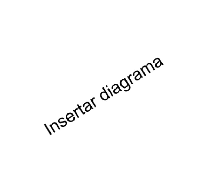
\includegraphics[width= 0.6\textwidth]{diagrama_secuencia01.png} 
\caption{\label{fig:seq01} Diagrama de Secuencia 1.}
\end{figure}


\begin{figure}[H]
	\centering
	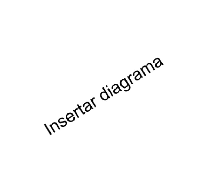
\includegraphics[width=0.6\textwidth]{diagrama_secuencia02.png}
	\caption{\label{fig:seq02} Diagrama de Secuencia 2.}
\end{figure}

\subsection{test04}

\begin{figure}[H]
  \centering
  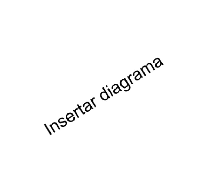
\includegraphics[width=0.6\textwidth]{diagrama_secuencia03.png}
  \caption{\label{fig:seq03}Diagrama de Secuencia del test04.}
  \end{figure}

  \begin{figure}[H]
    \centering
    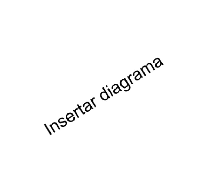
\includegraphics[width=0.6\textwidth]{diagrama_secuencia04.png}
    \caption{\label{fig:seq04}Diagrama de Secuencia.}
    \end{figure}



% \footnote{Mensaje debajo}

\begin{figure}[H]
  \centering
  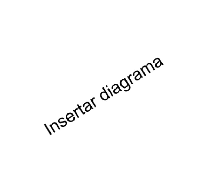
\includegraphics[width=0.6\textwidth]{diagrama_clase01.png}
  \caption{\label{fig:class01}Diagrama de Clases 1.}
  \end{figure}

  Descripcion del diagrama de Clase 1
  
\begin{figure}[H]
\centering
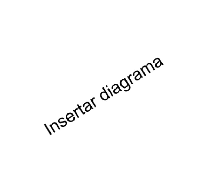
\includegraphics[width=0.6\textwidth]{diagrama_clase02.png}
\caption{\label{fig:class02}Diagrama de Clases 2.}
\end{figure}

Descripcion del diagrama de Clase 2


\section{Diagramas de Paquetes}\label{sec:diagramasdepaquetes}


\section{Diagramas de Estado}\label{sec:diagramasdeestado}

% Explicaciones sobre la implementación interna de algunas clases que consideren que puedan llegar a resultar interesantes.
\section{Detalles de implementación}\label{sec:implementacion}



% Explicación de cada una de las excepciones creadas y con qué fin fueron creadas.
\section{Excepciones}\label{sec:excepciones}
\begin{description}
\item[Exception \underline{Excepcion1:}] Se lanza la excepción 1
\item[Exception \underline{Excepcion2:}] 
\end{description}


  \section{Conclusión}
  
 	Redactar conclusion.
\newpage
\section{Referencias}

\begin{itemize}
  \item UML gota a gota. Martin Fowler con Kendall Scott
  \item Texto de apoyo conceptual de Algoritmos y Programación III Facultad de Ingeniería de la Universidad de Buenos Aires. Carlos Fontela 2018
  \item Diagramas de Secuencia: \url{https://plantuml.com/sequence-diagram}
  \item Diagramas de Clase: \url{https://plantuml.com/class-diagram}
  \item Diagrama de Clase: \url{http://ogom.github.io/draw_uml/plantuml/}
  \item UML si o si: \url{https://campus.fi.uba.ar/mod/lesson/view.php id=98901&pageid=2105&startlastseen=no}
  \item Documentacion para la herramienta LaTex: \url{https://www.overleaf.com/learn/latex/Main_Page}
\end{itemize}

\end{document}